%!TEX root = index.tex
\chapter{Data}

This chapter sumarizes which data were used for implementation and testing of the module for air traffic control simulation in terminal area. The design and implementation of the module is general and can be used for simulation of any TMA sector but in order to test its functionality concrete sector description and air traffic scenario must be used. It was important to have all the data relevant to the test sector available because any of them missing would cause the whole scenario to be unusable.

\section{Hartsfield–Jackson Atlanta International Airport}

\begin{figure}[h]
    \centering
    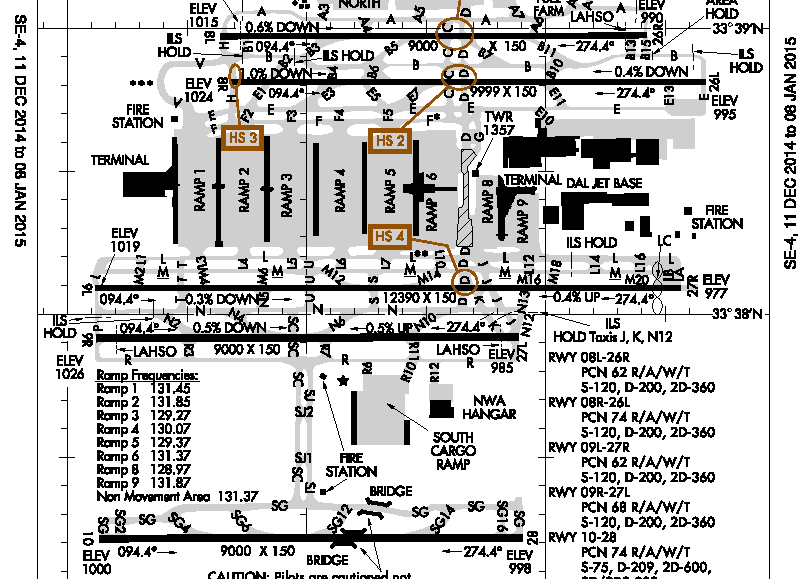
\includegraphics[width=0.8\textwidth]{figures/atlanta-diagram.pdf}
    \caption{Section of the airport diagram of the Hartsfield–Jackson Atlanta International Airport \cite{atlanta-diagram}}
    \label{fig:atlanta-diagram}
\end{figure}

Hartsfield–Jackson Atlanta International Airport (ICAO code KATL) has been the world's busiest airport by passenger traffic since 1998 with more than 94 million passengers in 2013. It has also the most landings and take-offs since 2005. The airport has 207 domestic and international gates which is the most at any airport. \cite{atlanta}

This airport was chosen because the amount of traffic would provide more interesting test-case in comparison to some other, less busy airport. Also all the other required data were available for Atlanta Airport.

The goal of this thesis is to simulate the approach phase of the flight, from the moment airplane leaves en-route sector to touchdown on the runway. The ground movement is not simulated and therefore the only information needed about the airport is the configuration of its runways.

The runway configuration is publicly available on the FAA website \cite{atlanta-diagram}. Airport runway configuration including positions and elevations of each runway was created in a form of XML file that can be used in AgentFly simulation.

The Atlanta Airport has five runways, the southernmost (\texttt{10/28}) is used for cargo aircraft and was therefore eliminated from the scenario. Out of the four remaining runways the inner two (\texttt{8R/26L} and \texttt{9L/27R}) are used exclusively for departures and only the outer two runways (\texttt{8L/26R} and \texttt{9R/27L}) are used for incomming flights. These two runways will be used in the test simulation scenarios. Figure \ref{fig:routes} shows all the Atlanta Airport runways as they are shown in AgentFly visualization.

\section{Atlanta TMA}

\begin{figure}[h]
    \centering
    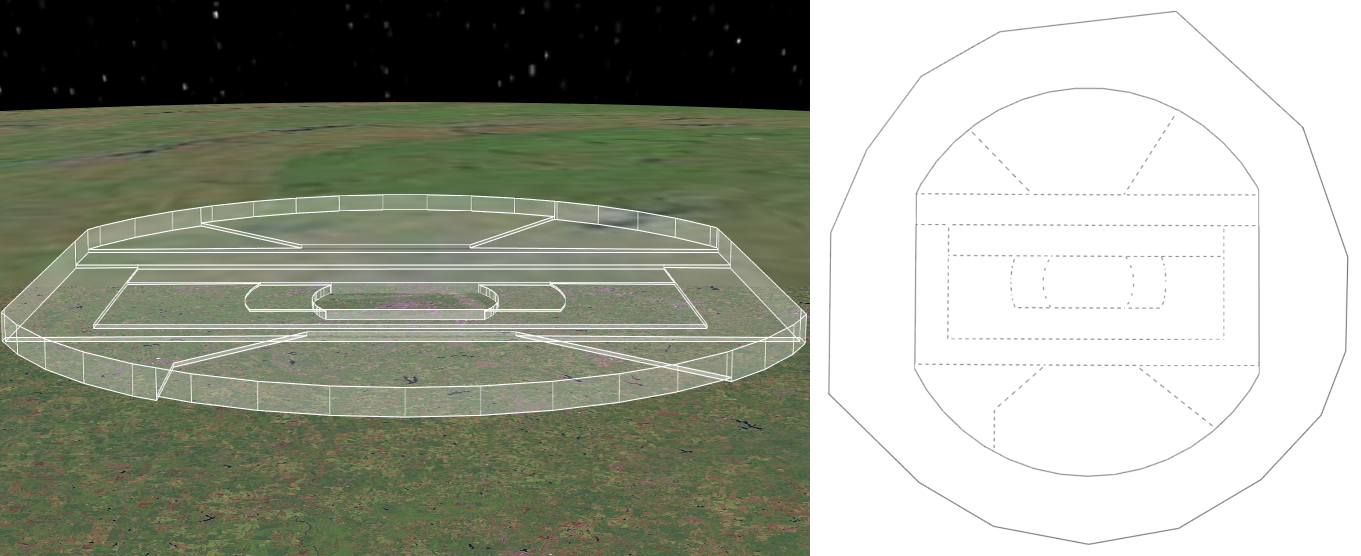
\includegraphics[width=\textwidth]{figures/tracon.png}
    \caption{\red{TODO: popis}}
    \label{fig:tracon}
\end{figure}


\section{SID + STARs}

\begin{figure}[h]
    \centering
    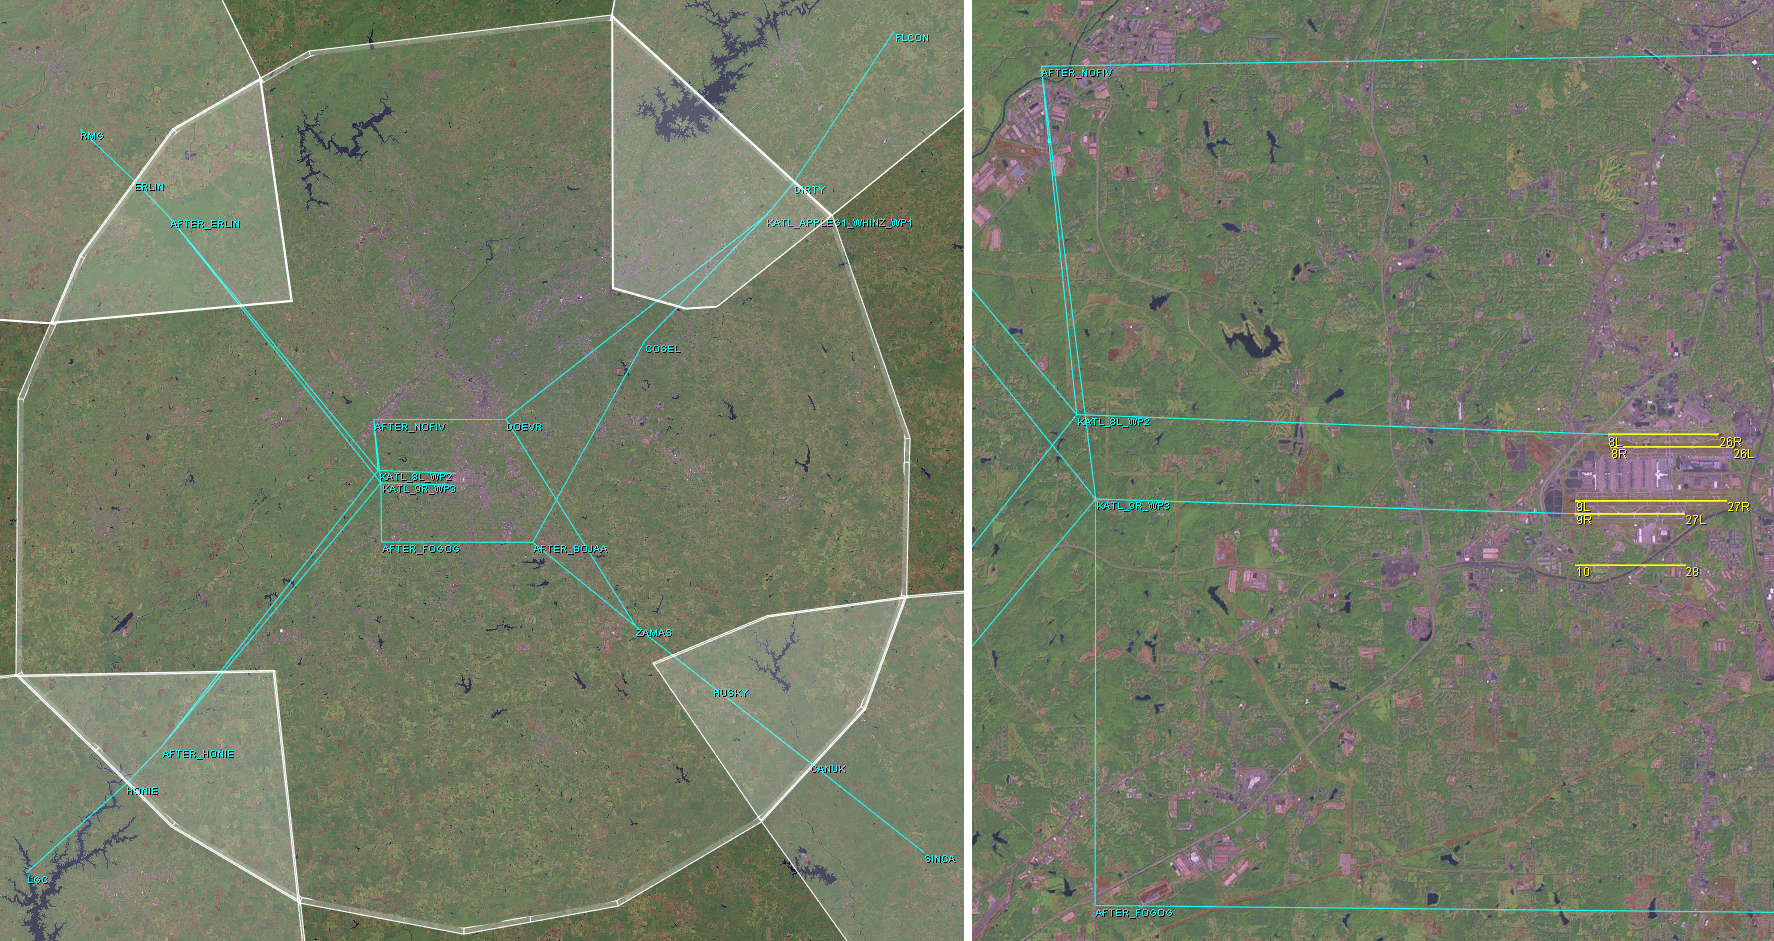
\includegraphics[width=\textwidth]{figures/routes.png}
    \caption{\red{TODO: popis}}
    \label{fig:routes}
\end{figure}

\section{Flights}

\begin{figure}[h]
    \centering
    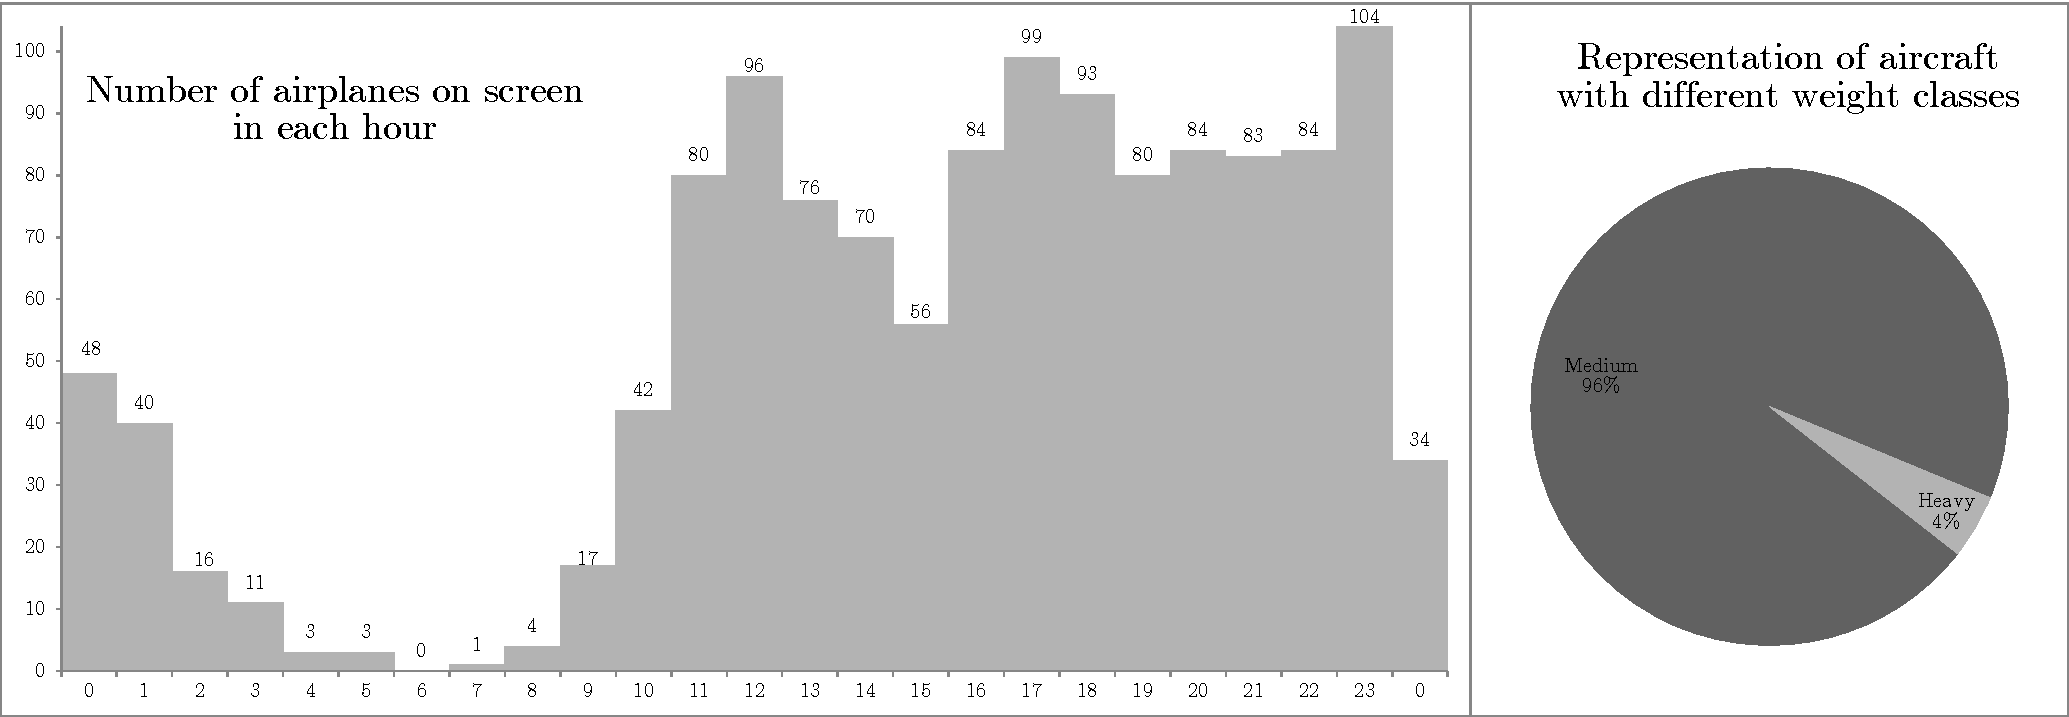
\includegraphics[width=\textwidth]{graphs/real-flights_scissored.pdf}
    \caption{\red{TODO: popis}}
    \label{graph:flights}
\end{figure}

% v agentfly počítáme pouze s  \item[IFR] Instrument flight rules lety \item[VFR] visual flight rules nás nezajímají

% %\textcolor{red}{v každou chvíli řídí letadlo jeden subjekt a místo a čas předání kontroly je jesně definované - kdy a jak?}


% %\textcolor{red}{Pro řízení v terminální oblasti nás zajímají všechny druhy řízení/prostoru, Agentfly má zatím jen ACC v CTA?}

% do implementace : proč používáme které classes v agentfly

